% command to make sure colorboxes don't create whitespace between code lines
\fboxsep=.6pt

% default settings for listings
\lstset{style=python, basicstyle=\ttfamily\footnotesize}

\title[Algorithmen]{Laufzeitkomplexität}

\author[Graf, Thomas] % (optional)
{Thomas Graf}

\institute[KLW] % (optional)
{
	Fachschaft Informatik\\
	Kantonsschule Im Lee
}

\date[\today] % (optional)

\logo{
\includegraphics[width=2cm]{Logos/LeeLogo}}

\titlegraphic{\vspace{-.7cm}\includegraphics[width=\textwidth]{"Grundlagen_Info/06_Datenbanken/Figures/title-emojis"}}

\frame{\titlepage}

\begin{frame}{Motivation}
	\begin{itemize}[<+->]
		\item Bislang stand für uns hauptsächlich die Frage
		\begin{center}
			{\small
			\enquote{Wie können wir ein Problem \textbf{überhaupt} algorithmisch lösen?}
			}
		\end{center}
		im Zentrum.
		\item Dabei haben wir uns (grob gesagt) \textbf{mit jeder korrekten algorithmischen Lösung begnügt}.
	\end{itemize}
\end{frame}


\begin{frame}{Diskussion im Plenum}
	Welche Aspekte eines Algorithmus könnten uns (neben seiner Korrektheit) noch interessieren?
	\pause
	\begin{itemize}[<+->]
		\item Eleganz?
		\item Effizienz?
		\item Lesbarkeit und Verständlichkeit?
		\item Länge des Codes? (Anzahl Zeilen / Zeichen)
	\end{itemize}
\end{frame}


\begin{frame}{Diskussion im Plenum}
	Welche Aspekte eines Algorithmus könnten uns (neben seiner Korrektheit) noch interessieren?
	\pause
	\begin{itemize}
		\item Eleganz
		\item \textcolor{Red}{\textbf{Effizienz}} $\leftarrow$ unser Fokus für heute
		\item Lesbarkeit und Verständlichkeit
		\item Länge des Codes (Anzahl Zeilen)
	\end{itemize}
\end{frame}


\begin{frame}{Effizienz (Laufzeit) ist eine wichtige Eigenschaft eines Algorithmus}
	\begin{itemize}[<+->]
		\item Kollisionserkennung: Unterschiede in den Framerates
		\item Google: \enquote{Loading times longer than a blink of an eye (or 400 milliseconds) are too long}:\\
		\url{https://current360.com/400-milliseconds-or-the-blink-of-an-eye/}
		\item Demonstration: Vergleich der Laufzeiten von \texttt{bubble\_sort} und \texttt{merge\_sort}
		% \item In den sechziger Jahren stellte man fest, dass alleine die Existenz eines Algorithmus zur Lösung eines Problems noch keine Garantie für eine erfolgreiche Computerberechnung des Problems darstellt!
		% \item Die Rechner stürzten häufig ab, bevor sie die Berechnung beenden konnten.
	\end{itemize}
\end{frame}

\begin{frame}{Lernziele}
	\begin{itemize}[<+->]
		\item Sie besitzen eine intuitive Vorstellung für die Komplexität alltäglicher algorithmischer Szenarien.
		\item Sie können die Begriffe \emph{Worst-Case} und \emph{Best-Case} erklären.
		\item Sie können die Laufzeit einfacher Algorithmen bestimmen.
	\end{itemize}
\end{frame}

\begin{frame}{Bestimmung der Laufzeit \faStar\faStar[regular]\faStar[regular]\faStar[regular]\faStar[regular]}
	\begin{myexercise}
    \lstinputlisting[basicstyle=\footnotesize\ttfamily,language=Python,caption=\texttt{a.py},label=listing:a]{EF/Complexity/Code/a.py}
    
    Wie oft wird die Funktion \lstinline{print} aufgerufen?
	\end{myexercise}
\end{frame}

\begin{frame}
\begin{myanswer}
    Die Funktion \lstinline{print} wird $5\cdot 4 = 20$ mal aufgerufen.
\end{myanswer}
\end{frame}

\begin{frame}{Bestimmung der Laufzeit \faStar\faStar[regular]\faStar[regular]\faStar[regular]\faStar[regular]}
	\begin{myexercise}
	\lstinputlisting[basicstyle=\footnotesize\ttfamily,language=Python,caption=\texttt{b.py},label=listing:b]{EF/Complexity/Code/b.py}

	Wie oft wird die Funktion \lstinline{print} aufgerufen?
	\end{myexercise}
\end{frame}

\begin{frame}
\begin{myanswer}
	Die Funktion \lstinline{print} wird $n^2$ mal aufgerufen.
\end{myanswer}
\end{frame}

\begin{frame}{Bestimmung der Laufzeit \faStar\faStar\faStar[regular]\faStar[regular]\faStar[regular]}
	\begin{myexercise}
	\lstinputlisting[basicstyle=\footnotesize\ttfamily,language=Python,caption=\texttt{c.py},label=listing:c,numbers=left]{EF/Complexity/Code/c.py}

	Wie oft wird das \lstinline{if}-Statement ausgeführt? \emoji{thinking-face}
	\end{myexercise}
\end{frame}

\begin{frame}
\begin{myanswer}
	Die genaue Anzahl hängt von der konkreten \textbf{Probleminstanz} -- in diesem Fall von der gegebenen Liste \lstinline{L} -- ab. Wir unterscheiden zwei extreme Fälle:
	\pause
	\begin{description}[<+->]
		\item[Günstigster Fall (Best-Case):] Das erste Element (\lstinline{L[0]}) ist bereits das gesuchte Element \lstinline{x} $\Rightarrow$ das \lstinline{if}-Statement wird nur einmal ausgeführt.
		\item[Teuerster Fall (Worst-Case):] Das gesuchte Element \lstinline{x} ist entweder das letzte Element der Liste oder kommt in der Liste gar nicht vor $\Rightarrow$ das \lstinline{if}-Statement wird \lstinline{n = len(L)} mal ausgeführt (jedes Element von \lstinline{L} muss überprüft werden).
	\end{description}
	\pause
	Natürlich können auch alle Fälle zwischen diesen beiden Extremfällen (1 bis \lstinline{len(L)} Ausführungen) auftreten.
\end{myanswer}
\end{frame}

\begin{frame}{\emph{Worst-Case} und \emph{Best-Case}}
	\begin{itemize}[<+->]
		\item Die \emph{Worst-Case} Laufzeit $T_{\text{worst}}(n)$ ist die maximale Anzahl der Operationen, die ein Algorithmus $A$ für eine Eingabe (Probleminstanz) der Grösse $n$ benötigt.
		\item Die \emph{Best-Case} Laufzeit $T_{\text{best}}(n)$ ist die minimale Anzahl der Operationen, die ein Algorithmus $A$ für eine Eingabe (Probleminstanz) der Grösse $n$ benötigt.
	\end{itemize}
\end{frame}

\begin{frame}
\begin{myremark}
	$T_{\text{worst}}(n)$ ist die \textbf{obere Schranke}: Sie garantiert, dass der Algorithmus $A$ für \textbf{jede} Probleminstanz der Grösse $n$ nach spätestens dieser Anzahl an Operationen fertig ist.
\end{myremark}
\end{frame}

\begin{frame}{Bestimmung der Laufzeit \faStar\faStar\faStar[regular]\faStar[regular]\faStar[regular]}
	\begin{myexercise}
	\lstinputlisting[basicstyle=\footnotesize\ttfamily,language=Python,caption=\texttt{d.py},label=listing:d,numbers=left]{EF/Complexity/Code/d.py}

	Wie oft wird die Zeile \lstinline{i *= 2} ungefähr ausgeführt?
	\end{myexercise}
\end{frame}

\begin{frame}
	\begin{myanswer}
	Wir beginnen mit \lstinline{i = 1} und \lstinline{i} wird in jedem Durchlauf der \lstinline{while}-Schleife verdoppelt. Wie häufig können wir den Wert von \lstinline{i} verdoppeln, bis die \lstinline{while}-Bedingung \lstinline{i <= n} nicht mehr erfüllt ist? Ungefähr $\log_2(n)$ mal.
	% \pause
	% \vspace{1cm}
	% {\small
	% Exakte Analyse: Die Zeile \lstinline{i *= 2} wird $\ceil{\log_2(n)} + 1$ mal ausgeführt.
	% }
	\end{myanswer}
\end{frame}

\begin{frame}{Aufgaben Teil 1 auf Moodle}
	Sie finden die Aufgaben unter \texttt{Moodle} $\rightarrow$ \texttt{Theorie} $\rightarrow$ \texttt{Laufzeitkomplexität}.
	\pause
	\begin{itemize}[<+->]
		\item Lösen Sie die \textcolor{Blue}{\textbf{Aufgaben Teil 1}} (Bearbeitungszeit: 20 Minuten).
		\item Bearbeiten Sie die Aufgaben alleine.
	\end{itemize}
\end{frame}

\begin{frame}[fragile]{Typisches Problem: \enquote{alle mit allen}}
	\begin{itemize}[<+->]
		\item Stellen Sie sich vor, $n$ Personen stossen bei einem Fest miteinander an.
		\item Jede Person stösst mit jeder anderen Person genau einmal an.
		\item Wie viele Anstösse (Begegnungen) gibt es insgesamt?
	\end{itemize}
	\pause
	\begin{figure}
		\centering
		\begin{tikzpicture}[scale=0.8]
			\foreach \i in {1,...,5} {
				\node[circle,fill=RoyalBlue!20,draw=RoyalBlue,thick,minimum size=0.6cm] (p\i) at ({72*(\i-1)+90}:2cm) {\tiny \i};
			}
			\only<4>{
				\foreach \i in {1,...,4} {
					\pgfmathtruncatemacro{\nextj}{\i+1}
					\foreach \j in {\nextj,...,5} {
						\draw[gray!30,thin] (p\i) -- (p\j);
					}
				}
			}
			\only<5>{
				\draw[Red,thick] (p1) -- (p2);
				\draw[Red,thick] (p1) -- (p3);
				\draw[Red,thick] (p1) -- (p4);
				\draw[Red,thick] (p1) -- (p5);
				\node[anchor=west] at (2.5,1) {\textcolor{Red}{Person 1: $n-1$ Anstösse}};
			}
			\only<6>{
				\foreach \j in {2,3,4,5} \draw[gray!30,thin] (p1) -- (p\j);
				\draw[Orange,thick] (p2) -- (p3);
				\draw[Orange,thick] (p2) -- (p4);
				\draw[Orange,thick] (p2) -- (p5);
				\node[anchor=west] at (2.5,0) {\textcolor{Orange}{Person 2: $n-2$ neue Anstösse}};
			}
			\only<7>{
			    \foreach \j in {2,...,5} \draw[gray!30,thin] (p1) -- (p\j);
			    \foreach \j in {3,...,5} \draw[gray!30,thin] (p2) -- (p\j);
			    \draw[ForestGreen,thick] (p3) -- (p4);
			    \draw[ForestGreen,thick] (p3) -- (p5);
			    \node[anchor=west] at (2.5,-1) {\textcolor{ForestGreen}{Person 3: $n-3$ neue Anstösse}};
			}
			\only<8->{
			    \foreach \j in {2,...,5} \draw[gray!30,thin] (p1) -- (p\j);
			    \foreach \j in {3,...,5} \draw[gray!30,thin] (p2) -- (p\j);
			    \foreach \j in {4,...,5} \draw[gray!30,thin] (p3) -- (p\j);
			    \draw[Violet,thick] (p4) -- (p5);
			    \node[anchor=west] at (2.5,-2) {\textcolor{Violet}{Person 4: $n-4$ neue Anstösse}};
			}
		\end{tikzpicture}
	\end{figure}
    \only<9->{
	Insgesamt haben wir also $(n-1) + (n-2) + (n-3) + \ldots + 1$ Anstösse.
    }
\end{frame}

\begin{frame}{\enquote{alle mit allen}}
	\begin{itemize}[<+->]
		\item Die Summe $(n-1) + (n-2) + (n-3) + \ldots + 1$ ist Ihnen wohlbekannt!
		\item $(n-1) + (n-2) + (n-3) + \ldots + 1 \stackrel{\text{Gausssche Summenformel}}{=} \frac{n(n-1)}{2}$
		\item Beachten Sie den \textcolor{Red}{quadratischen Term}: $\frac{n(n-1)}{2} = \frac{1}{2}\cdot\textcolor{Red}{n^2} - \frac{n}{2}$.
	\end{itemize}
\end{frame}

\begin{frame}{Situation: \enquote{alle mit allen}}
	\begin{myexercise}
		Das Prinzip \enquote{Jeder mit Jedem} begegnet uns an vielen Stellen im täglichen Leben. Wo tritt dieses Muster noch auf? Nennen Sie drei konkrete Situationen, in denen alle Beteiligten untereinander in Kontakt stehen.
	\end{myexercise}
\end{frame}

\begin{frame}
	\begin{myanswer} 
		{\small
		\begin{itemize}
			\item Tischtennisturnier: Jeder Spieler spielt genau einmal gegen jeden anderen Spieler.
			\item Fotos von Zweierpaaren: In einer Gruppe von Personen werden Fotos von allen möglichen Zweierpaaren gemacht.
			\item Freundschaftsnetzwerk: In einem sozialen Netzwerk schreibt jeder Nutzer eine Nachricht an jeden anderen Nutzer (vollständiger Graph):
			\begin{center}
				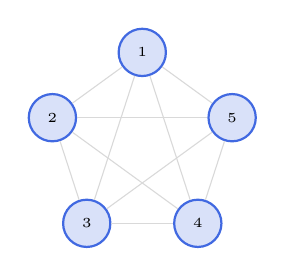
\begin{tikzpicture}[scale=0.6]
					\foreach \i in {1,...,5} {
						\node[circle,fill=RoyalBlue!20,draw=RoyalBlue,thick,minimum size=0.6cm] (p\i) at ({72*(\i-1)+90}:2cm) {\tiny \i};
					}
					\foreach \i in {1,...,4} {
						\pgfmathtruncatemacro{\nextj}{\i+1}
						\foreach \j in {\nextj,...,5} {
							\draw[gray!30,thin] (p\i) -- (p\j);
						}
					}
				\end{tikzpicture}
			\end{center}
		\end{itemize}
		}
	\end{myanswer}
\end{frame}

\begin{frame}{Aufgaben Teil 2 auf Moodle}
	Sie finden die Aufgaben unter \texttt{Moodle} $\rightarrow$ \texttt{Theorie} $\rightarrow$ \texttt{Laufzeitkomplexität}.
	\pause
	\begin{itemize}
		\item Lösen Sie die \textcolor{Blue}{\textbf{Aufgaben Teil 2}} (Bearbeitungszeit: 20 Minuten).
		\item Bearbeiten Sie die Aufgaben alleine oder zu zweit.
	\end{itemize}
\end{frame}

\begin{frame}
\begin{myexercise}
Gegeben sind zwei Algorithmen \(A\) und \(B\) für ein algorithmisches Problem.
\begin{itemize}
	\item Algorithmus \(A\): benötigt \(2^n\) Rechenoperationen,
	\item Algorithmus \(B\): benötigt \(n^2\) Rechenoperationen
\end{itemize}
zur Berechnung einer Lösung für eine Problemgrösse \(n\).
\vspace{0.3cm}

Eine Operation dauert genau 1 Mikrosekunde.
\vspace{0.5cm}

Wie gross darf $n$ maximal sein, damit die Berechnung in 24 Stunden fertig ist? (für $A$ und $B$)
\end{myexercise}
\end{frame}

\begin{frame}
\begin{myanswer}
\begin{itemize}[<+->]
	\item Algorithmus \(A\): Wir müssen die Ungleichung \(2^n \leq 24 \cdot 60 \cdot 60 \cdot 10^6\) lösen, da es $24 \cdot 60 \cdot 60 \cdot 10^6$ Mikrosekunden in 24 Stunden gibt. Das ergibt \(n \leq \log_2\lr{24 \cdot 60 \cdot 60 \cdot 10^6} \approx 36.33\Rightarrow \text{gesuchte Problemgrösse: } 36 \).
	\item Algorithmus \(B\): Wir müssen die Ungleichung \(n^2 \leq 24 \cdot 60 \cdot 60 \cdot 10^6\) lösen. Das ergibt \(n \leq \sqrt{24 \cdot 60 \cdot 60 \cdot 10^6} \approx 293938.77 \Rightarrow \text{gesuchte Problemgrösse: } 293938\).
\end{itemize}
\end{myanswer}
\end{frame}

\begin{frame}
\begin{myexercise}
Gegeben sind zwei Algorithmen \(A\) und \(B\) für ein algorithmisches Problem. In diesem Kontext existieren nur Problemgrössen \(n \in \N\), die \textbf{gerade} sind.
\begin{itemize}
	\item Algorithmus \(A\): benötigt \(4.5n + 15\) Rechenoperationen.
	\item Algorithmus \(B\): benötigt \(0.5n^2 + n\) Rechenoperationen.
\end{itemize}
Hinweis: Wir gehen davon aus, dass jede Rechenoperation die gleiche Zeit beansprucht.
\vspace{0.5cm}
Was ist die kleinste gerade Zahl \(n > 0\), für welche Algorithmus \(A\) das Problem schneller löst (also weniger Rechenoperationen benötigt) als Algorithmus \(B\)?
\end{myexercise}
\end{frame}

\begin{frame}
\begin{myanswer}
Wir müssen die Ungleichung \(4.5n + 15 < 0.5n^2 + n\) lösen. Das ergibt \(n^2 - 7n - 30 > 0\). Die Lösungen dieser Ungleichung sind \(n < -3\) sowie \(n > 10\). Da wir nur gerade Zahlen \(n > 0\) betrachten, ist die gesuchte Problemgrösse \(12\).
\end{myanswer}
\end{frame}

\begin{frame}{Bestimmung der Laufzeit \faStar\faStar\faStar[regular]\faStar[regular]\faStar[regular]}
	\begin{myexercise}
    \lstinputlisting[basicstyle=\small\ttfamily,language=Python,caption=\texttt{anstossen.py},label=listing:anstossen]{EF/Complexity/Code/anstossen.py}
 
    Wie oft wird die Funktion \lstinline{print} aufgerufen?
	\end{myexercise}
\end{frame}

\begin{frame}[fragile]
\begin{myanswer}
{\scriptsize
    Die Funktion \lstinline{print} wird
    \begin{itemize}[<+->]
        \item im ersten Durchlauf der äusseren Schleife (Fall \lstinline{i = 0}) genau \textcolor{orange}{$n-1$} mal,
        \item im zweiten Durchlauf der äusseren Schleife (Fall \lstinline{i = 1}) genau \textcolor{cyan}{$n-2$} mal,
        \item $\vdots$
        \item im letzten Durchlauf der äusseren Schleife (Fall \lstinline{i = n - 2}) genau \textcolor{magenta}{$1$} mal
    \end{itemize}
    \pause
    aufgerufen.

    \pause
    Total haben wir also
    \begin{align*}
		&\textcolor{magenta}{1} + 2 + 3 + \ldots + \textcolor{cyan}{(n-2)} + \textcolor{orange}{(n-1)} \stackrel{\text{Gausssche Summenformel}}{=} \frac{n(n-1)}{2} =\\
		&= \frac{1}{2}\cdot\textcolor{Red}{n^2} - \frac{n}{2}
	\end{align*}
	\pause
    Aufrufe von \lstinline{print}.
}%
\end{myanswer}
\end{frame}

\begin{frame}{Exakte Analyse eines Algorithmus}
	\begin{mydefinition}[Anzahl Wiederholungen pro Zeile]\label{mydefinition:wk}
	Bei einem gegebenen Algorithmus $A$, bezeichnen wir mit $w_k(n)$ die Anzahl der Ausführungen von Zeile $k$ bei Eingabegrösse $n$.
	\end{mydefinition}
\end{frame}

\begin{frame}[fragile]{Beispiel einer exakten Analyse (Problemgrösse $n$)}
    Wir analysieren ein einfaches Programm, das die Summe der ersten $n$ natürlichen Zahlen berechnet:
\begin{lstlisting}[escapechar=!,basicstyle=\footnotesize\ttfamily,numbers=left]
def berechne_summe(n): !\tikzmark{s1end}!                !\tikzmark{s1start}!
    s = 0 !\tikzmark{s2end}!                             !\tikzmark{s2start}!
    for i in range(n): !\tikzmark{s3end}!                !\tikzmark{s3start}!
        s = s + i !\tikzmark{s4end}!                     !\tikzmark{s4start}!
    return s !\tikzmark{s5end}!                          !\tikzmark{s5start}!
\end{lstlisting}
\begin{tikzpicture}[overlay, remember picture,
        every node/.style={draw=green!50,fill=green!35!white,text=black,rounded corners}]
    \only<2->{\drawArrow{s1end}{s1start}{\tiny $w_1(n) = 1$}{green!35!white};}
    \only<3->{\drawArrow{s2end}{s2start}{\tiny $w_2(n) = 1$}{green!35!white};}
    \only<4->{\drawArrow{s3end}{s3start}{\tiny $w_3(n) = n + 1$}{green!35!white};}
    \only<5->{\drawArrow{s4end}{s4start}{\tiny $w_4(n) = n$}{green!35!white};}
    \only<6->{\drawArrow{s5end}{s5start}{\tiny $w_5(n) = 1$}{green!35!white};}
\end{tikzpicture}
\end{frame}

\begin{frame}
\begin{itemize}[<+->]
    \item $w_3(n) = n+1$, da die \lstinline{for}-Schleife $n$ mal läuft und am Ende einmal die Abbruchbedingung prüft.
	\item Wir bezeichnen mit $c_k$ die Kosten (\textbf{c}ost) einer einmaligen Ausführung von Programmzeile $k$.
	\item Unter Kosten verstehen wir die Anzahl der elementaren Operationen, die in Zeile $k$ ausgeführt werden (z.\,B. Zuweisungen, Vergleiche, arithmetische Operationen, etc.).
	\item Wir nehmen an, dass die $c_k$ unabhängig von $n$ sind.
    \item Die Gesamtlaufzeit $T(n)$ ergibt sich aus den Kosten $c_k$ pro Zeile:
\end{itemize}
\end{frame}

\begin{frame}{Beispiel einer exakten Analyse (Fortsetzung)}
    Wir stellen die Formel für $T(n)$ auf:
    {\footnotesize
    \begin{align*}
        \onslide<2->{T(n) &= c_1w_1(n) + c_2w_2(n) + c_3w_3(n) + c_4w_4(n) + c_5w_5(n) =\\
        }
        \onslide<3->{&= c_1 + c_2 + c_3(n+1) + c_4n + c_5 =\\
        }
        \onslide<4->{&= \underbrace{(c_3 + c_4)}_{=:\textcolor{RoyalBlue}{a}}n + \underbrace{(c_1 + c_2 + c_3 + c_5)}_{=:\textcolor{ForestGreen}{b}} =\\
        }
        \onslide<5->{&= \textcolor{RoyalBlue}{a}n + \textcolor{ForestGreen}{b}}
    \end{align*}
    }
    \only<6->{
    \begin{myremark}
        Dieses Programm hat eine \textbf{lineare Laufzeit}.
    \end{myremark}
    }
\end{frame}

\begin{frame}{Aufgaben Teil 3 auf Moodle}
	Sie finden die Aufgaben unter \texttt{Moodle} $\rightarrow$ \texttt{Theorie} $\rightarrow$ \texttt{Laufzeitkomplexität}.
	\pause
	\begin{itemize}
		\item Lösen Sie die \textcolor{Blue}{\textbf{Aufgaben Teil 3}} (Bearbeitungszeit: 8 Minuten).
		\item Bearbeiten Sie die Aufgaben alleine oder zu zweit.
	\end{itemize}
\end{frame}

\begin{frame}[fragile]{Analyse von \texttt{bubble\_sort} für Problemgrösse $n$, \textcolor{Red}{Worst-Case}}
\begin{lstlisting}[escapechar=!,basicstyle=\footnotesize\ttfamily,numbers=left]
def bubble_sort(A): !\tikzmark{c1end}! 								!\tikzmark{c1start}!
    n = len(A) !\tikzmark{c2end}! 									!\tikzmark{c2start}!
    for i in range(n - 1): !\tikzmark{c3end}! 						!\tikzmark{c3start}!
        for j in range(n - i - 1): !\tikzmark{c4end}! 				!\tikzmark{c4start}!
            if A[j] > A[j + 1]:	!\tikzmark{c5end}! 					!\tikzmark{c5start}!
                A[j], A[j+1] = A[j+1], A[j] !\tikzmark{c6end}! 		!\tikzmark{c6start}!
    return A !\tikzmark{c7end}!										!\tikzmark{c7start}!
\end{lstlisting}
\begin{tikzpicture}[overlay, remember picture,
        every node/.style={draw=green!50,fill=green!35!white,text=black,rounded corners}]
    % Each arrow will appear one after another
    \only<2->{\drawArrow{c1end}{c1start}{\tiny $w_1(n) = 1$}{green!35!white};}
    \only<3->{\drawArrow{c2end}{c2start}{\tiny $w_2(n) = 1$}{green!35!white};}
    \only<4->{\drawArrow{c3end}{c3start}{\tiny $w_3(n) = n$}{green!35!white};}
    \only<8->{\drawArrow{c4end}{c4start}{\tiny $w_4(n) = w_5(n) + n - 1$}{green!35!white};}
    \only<5->{\drawArrow{c5end}{c5start}{\tiny $w_5(n)$}{green!35!white};}
    \only<6->{\drawArrow{c6end}{c6start}{\tiny $w_6(n) = w_5(n)$}{red!55!white};}
    \only<7->{\drawArrow{c7end}{c7start}{\tiny $w_7(n) = 1$}{green!35!white};}
\end{tikzpicture}
\end{frame}

\begin{frame}[fragile]{Analyse von \texttt{bubble\_sort} für Problemgrösse $n$, \textcolor{Red}{Worst-Case}}
\begin{itemize}[<+->]
	\item Der \textcolor{Red}{Worst-Case} liegt vor, wenn die gegebene Liste \textbf{absteigend} sortiert ist (z.\,B. \lstinline{A = [9, 5, 3, 0]}).
	\item Im \textcolor{Red}{Worst-Case} müssen die Elemente in \textbf{jedem} inneren Schleifendurchlauf getauscht werden $\Rightarrow w_6(n) = w_5(n)$.
	\item $w_4(n)$ ist grösser als $w_5(n)$, da die \lstinline{for}-Bedingung pro äusserem Durchlauf einmal öfter geprüft wird (Abbruchprüfung).
\end{itemize}
\end{frame}

\begin{frame}[fragile]{Genaue Analyse von \texttt{bubble\_sort}, \textcolor{Red}{Worst-Case}}
\lstinputlisting[basicstyle=\scriptsize\ttfamily,language=Python,caption=\texttt{bubble\_sort.py},label=listing:bubble_sort,numbers=left]{EF/Complexity/Code/bubble_sort.py}
{\footnotesize
Wir müssen nun die totale Anzahl der Ausführungen von Zeile 5, also $w_5(n)$, bestimmen:
\pause
\begin{itemize}[<+->]
	\item Wenn \lstinline{i = 0}, läuft \lstinline{j} von \lstinline{0} bis \lstinline{n - 2} $\Rightarrow$ $(n-1)$ Mal
	\item Wenn \lstinline{i = 1}, läuft \lstinline{j} von \lstinline{0} bis \lstinline{n - 3} $\Rightarrow$ $(n-2)$ Mal
	\item $\vdots$
	\item Wenn \lstinline{i = n - 2}, läuft \lstinline{j} von \lstinline{0} bis \lstinline{0}, wegen \lstinline{range(0, 1)} $\Rightarrow$ $1$ Mal
\end{itemize}
\pause
Wir erhalten die bekannte Summe:
{\scriptsize
\begin{align*}
	w_5(n) = (n-1) + (n-2) + \ldots + 1 = \frac{n(n-1)}{2} = \frac{n^2}{2} - \frac{n}{2}.
\end{align*}
}
}
\end{frame}

\begin{frame}[fragile]{Genaue Analyse von \texttt{bubble\_sort}, \textcolor{Red}{Worst-Case}}
\phantom{1}
{\footnotesize
\begin{align*}
	T_{\text{worst}}(n) &= c_1w_1(n) + c_2w_2(n) + \ldots + c_7w_7(n) = \\
	&= c_1 + c_2 + c_3(n) + c_4\left(w_5(n) + n-1\right) + c_5w_5(n) + c_6w_5(n) + c_7 = \\
	&= c_1 + c_2 + c_3n + c_4\left(\frac{n(n-1)}{2}+n-1\right) + (c_5+c_6)\left(\frac{n(n-1)}{2}\right) + c_7
\end{align*}
}
\end{frame}

\begin{frame}[fragile]{Genaue Analyse von \texttt{bubble\_sort}}
	Wir vereinfachen die Terme und gruppieren nach den Potenzen von $n$, um den folgenden Ausdruck zu erhalten:
	\pause
{\footnotesize
\begin{align*}
T_{\text{worst}}(n) &= \underbrace{\left(\frac{c_4 + c_5 + c_6}{2}\right)}_{=:\textcolor{Red}{a}} n^2 + \underbrace{\left(c_3 + \frac{c_4 - c_5 - c_6}{2}\right)}_{=:\textcolor{RoyalBlue}{b}}n + \underbrace{(c_1 + c_2 - c_4 + c_7)}_{=:\textcolor{ForestGreen}{c}} = \\
&= \textcolor{Red}{a}n^2 + \textcolor{RoyalBlue}{b}n + \textcolor{ForestGreen}{c}
\end{align*}}
\end{frame}

\begin{frame}{Challenge-Aufgaben auf Moodle}
	Sie finden die Aufgaben unter \texttt{Moodle} $\rightarrow$ \texttt{Theorie} $\rightarrow$ \texttt{Laufzeitkomplexität}.\\
	\vspace{1.0cm}	
	Lösen Sie die \textcolor{Blue}{\textbf{Challenge-Aufgaben}}.
\end{frame}


\begin{frame}[fragile]{Analyse von \texttt{insertion\_sort}}
	\begin{myexercise}
		{\small
		Führen Sie eine vollständige Laufzeitanalyse von \texttt{insertion\_sort} für den \textbf{Worst-Case} durch:
		}
		\lstinputlisting[language=Python,caption=\texttt{insertion\_sort.py},numbers=left]{EF/Complexity/Code/insertion_sort.py}
	\end{myexercise}
\end{frame}

\begin{frame}
	\begin{myanswer}
		Im Worst-Case muss jedes Element mit allen vorherigen Elementen verglichen werden. Das Element bei Index $j$ wird $j+1$ Mal in der \lstinline{while}-Bedingung überprüft.
	\end{myanswer}
\end{frame}

\begin{frame}[fragile]
\begin{myanswer}
\begin{lstlisting}[escapechar=!,basicstyle=\footnotesize\ttfamily,numbers=left]
def insertion_sort(A): !\tikzmark{c1end}! 						!\tikzmark{c1start}!
    n = len(A) !\tikzmark{c2end}! 								!\tikzmark{c2start}!
    for j in range(1, n): !\tikzmark{c3end}! 						!\tikzmark{c3start}!
        key = A[j] !\tikzmark{c4end}! 							!\tikzmark{c4start}!
        i = j - 1	!\tikzmark{c5end}! 							!\tikzmark{c5start}!
		while i >= 0 and A[i] > key: !\tikzmark{c6end}! 			!\tikzmark{c6start}!
			A[i + 1] =  A[i] !\tikzmark{c7end}! 					!\tikzmark{c7start}!
			i -= 1 !\tikzmark{c8end}! 							!\tikzmark{c8start}!
		A[i + 1] = key !\tikzmark{c9end}!	 						!\tikzmark{c9start}!
    return A !\tikzmark{c10end}!									!\tikzmark{c10start}!
\end{lstlisting}
\begin{tikzpicture}[overlay, remember picture,
        every node/.style={draw=green!50,fill=green!35!white,text=black,rounded corners}]
    % Each arrow will appear one after another on mouse click
    \only<2->{\drawArrow{c1end}{c1start}{\tiny $w_1(n) = 1$}{green!35!white};}
    \only<3->{\drawArrow{c2end}{c2start}{\tiny $w_2(n) = 1$}{green!35!white};}
    \only<4->{\drawArrow{c3end}{c3start}{\tiny $w_3(n) = n$}{green!35!white};}
    \only<5->{\drawArrow{c4end}{c4start}{\tiny $w_4(n) = n-1$}{green!35!white};}
    \only<6->{\drawArrow{c5end}{c5start}{\tiny $w_5(n) = n-1$}{green!35!white};}
    \only<11->{\drawArrow{c6end}{c6start}{\tiny $w_6(n) = w_7(n) + (n-1)$}{green!35!white};}
    \only<7->{\drawArrow{c7end}{c7start}{\tiny $w_7(n)$}{green!35!white};}
    \only<8->{\drawArrow{c8end}{c8start}{\tiny $w_8(n) = w_7(n)$}{green!35!white};}
    \only<9->{\drawArrow{c9end}{c9start}{\tiny $w_9(n) = n-1$}{green!35!white};}
    \only<10->{\drawArrow{c10end}{c10start}{\tiny $w_{10}(n) = 1$}{green!35!white};}
\end{tikzpicture}
\end{myanswer}
\end{frame}

\begin{frame}
\begin{myanswer}
\begin{align*}
w_7(n) = 1 + 2 + \ldots + (n-1) = \frac{n(n-1)}{2}
\end{align*}
Für jeden der $n-1$ Durchläufe der äusseren Schleife muss im Kopf der \lstinline{while}-Schleife am Ende noch einmal die Abbruch-Bedingung überprüft werden $\Rightarrow w_6(n) = w_7(n) + (n-1)$.
\end{myanswer}
\end{frame}

\begin{frame}
\begin{myanswer}
Zusammengefasst erhalten wir:
{\scriptsize
\begin{align*}
\tilde{T}_{\text{worst}}(n) &= \tilde{c}_1w_1(n) + \tilde{c}_2w_2(n) + \ldots + \tilde{c}_{10}w_{10}(n) = \sum_{k=1}^{10}\tilde{c}_kw_k(n) = \\
&= \tilde{c}_1 + \tilde{c}_2 + \tilde{c}_3n + \tilde{c}_4(n-1) + \tilde{c}_5(n-1) +\\
&+ \tilde{c}_6\lr{\frac{n(n-1)}{2}+(n-1)} + \tilde{c}_7\lr{\frac{n(n-1)}{2}} +\\
&+ \tilde{c}_8\lr{\frac{n(n-1)}{2}} + \tilde{c}_9(n-1) + \tilde{c}_{10}
\end{align*}
}
\end{myanswer}
\end{frame}

\begin{frame}
\begin{myanswer}
{\scriptsize
Wir vereinfachen die Terme und gruppieren nach den Potenzen von $n$, um den folgenden Ausdruck zu erhalten:
\begin{align*}
\tilde{T}_{\text{worst}}(n) &= \underbrace{\lr{\frac{\tilde{c}_6 + \tilde{c}_7 + \tilde{c}_8}{2}}}_{=:\textcolor{Red}{\tilde{a}}} n^2 +\\
&+ \underbrace{\lr{\tilde{c}_3 + \tilde{c}_4 + \tilde{c}_5 + \frac{\tilde{c}_6 - \tilde{c}_7 - \tilde{c}_8}{2} + \tilde{c}_9}}_{=:\textcolor{RoyalBlue}{\tilde{b}}}n +\\
&+ \underbrace{\lr{\tilde{c}_1 + \tilde{c}_2 - \tilde{c}_4 - \tilde{c}_5 - \tilde{c}_6 - \tilde{c}_9 + \tilde{c}_{10}}}_{=:\textcolor{ForestGreen}{\tilde{c}}}=\\
&= \textcolor{Red}{\tilde{a}}n^2 + \textcolor{RoyalBlue}{\tilde{b}} + \textcolor{ForestGreen}{\tilde{c}}
\end{align*}
}
\end{myanswer}
\end{frame}


% \begin{frame}{Berechenbarkeit}
% 	\begin{itemize}[<+->]
% 		\item Die Theorie der Berechenbarkeit liefert uns Methoden zur Klassifizierung von Problemen bezüglich ihrer algorithmischen Lösbarkeit. Danach ist ein Problem \textbf{\textcolor{Green}{algorithmisch lösbar}}, wenn ein Algorithmus zur Lösung dieses Problems existiert, und ein Problem ist \textbf{\textcolor{Red}{algorithmisch unlösbar}}, wenn kein Algorithmus für dieses Problem existiert.
% 		\item Wir werden uns in diesem Thema auf \textbf{\textcolor{Green}{algorithmisch lösbare}} Probleme beschränken.
% 		\item Könnt ihr euch noch an ein Beispiel eines algorithmisch unlösbaren Problems erinnern?
% 	\end{itemize}
% \end{frame}

% \begin{frame}{Komplexitätstheorie}
% 	\begin{itemize}[<+->]
% 		\item In den sechziger Jahren stellte man fest, dass alleine die Existenz eines Algorithmus zur Lösung eines Problems noch keine Garantie für eine erfolgreiche rechnerunterstützte Lösung des Problems darstellt!
% 		\item Es waren zahlreiche praxisrelevante algorithmische Probleme bekannt, die zwar grundsätzlich algorithmisch lösbar waren, aber für die alle entworfenen Programme tagelang auf gegebenen Eingaben ohne Erfolg arbeiteten. Die Rechner stürzten häufig ab, bevor sie die Berechnung beenden konnten.
% 		\item Die Komplexitätstheorie strebt eine feinere Einteilung der algorithmisch lösbaren Probleme an.
% 	\end{itemize}
% \end{frame}

% \begin{frame}{Komplexitätstheorie}
% 	\begin{itemize}[<+->]
% 		\item Es stellte sich die Frage, ob dieser Misserfolg eine Folge unserer Unfähigkeit ist, einen effizienten Ansatz zur Lösung des betrachteten Problems zu finden, oder aber, ob es sich um eine \textbf{inhärente Eigenschaft des Problems} handelt, die keine effiziente algorithmische Lösung des Problems zulässt.
% 		\item Dies führte dazu, dass man begann, die Schwierigkeit der algorithmisch lösbaren Probleme bezüglich des Rechenaufwands zu messen, um so die Probleme nach deren Schwierigkeitsgrad zu klassifizieren.
% 	\end{itemize}
% \end{frame}

% \begin{frame}{Komplexitätstheorie}
% 	Die Komplexitätstheorie ist die Theorie der quantitativen Gesetze und Grenzen der algorithmischen Informationsverarbeitung. Diese Theorie hat auch eine physikalische Dimension: Zum Beispiel hält man ein zwar berechenbares Problem sicherlich für \enquote{praktisch unlösbar}, wenn die Ausführung eines Algorithmus zur Lösung des Problems mehr Energie bräuchte, als im bekannten Universum vorhanden ist.
% \end{frame}


% \begin{frame}{worst-case}
% 	Den schwierigsten / schlimmsten Probleminstanzen (Fällen) kommt in der Informatik eine besondere Bedeutung zu. Man spricht von der \textit{Laufzeit im Schlimmsten Fall} (englisch: \textit{worst-case running time}). Die Idee hinter diesem Ansatz ist offensichtlich: In der Zeit in der wir diese schlimmsten Fälle berechnen können, können wir erst recht alle anderen Fälle berechnen.
% \end{frame}

% \begin{frame}{worst-case für \texttt{insertion\_sort}}
% 	Wir bezeichnen mit $T(n)$ die maximale Laufzeit, welche unser \texttt{insertion\_sort} Algorithmus benötigt, um jede (auch die schwierigste) Probleminstanz der Grösse $n$ (hier: zu sortierende Liste der Länge $n$) zu lösen (zu sortieren). Es gilt also:
% 	{\scriptsize
% 		\begin{align*}
% 			T(n) = \max\lrc{\settt{Laufzeit von \texttt{insertion\_sort} auf $A$}{$A$ ist eine Liste der Länge $n$}}.
% 		\end{align*}
% 	}
% \end{frame}

\begin{frame}{Das Modell der Random Access Machine (RAM)}
	\begin{itemize}[<+->]
		\item Um die Laufzeit von Algorithmen präzise und unabhängig von konkreter Hardware zu analysieren, verwenden wir ein abstraktes Computermodell: die \textbf{Random Access Machine (RAM)}.
		\item Bisher war unsere Analyse mit Kosten $c_k$ pro Zeile zwar exakt, aber auch aufwendig. Das RAM-Modell vereinfacht die Analyse erheblich.
		\item Die RAM ist ein idealisierter Computer (ähnlich der Von-Neumann-Architektur) mit folgenden Eigenschaften:
		\begin{itemize}
			\item \textbf{Speicher:} Genügend viele Speicherzellen, auf die direkt zugegriffen werden kann (Random Access).
			\item \textbf{Programm:} Eine Folge von einfachen Befehlen (elementare Operationen), die sequentiell abgearbeitet werden.
		\end{itemize}
	\end{itemize}
\end{frame}

\begin{frame}{Kostenmodell der RAM}
	\begin{itemize}[<+->]
		\item Wie messen wir die \enquote{Zeit} in diesem Modell?
		\item Wir verwenden das \textbf{Einheitskostenmodell (Uniform Cost Model):}
		\begin{itemize}
			\item Jede elementare Operation (Addition, Subtraktion, Vergleich, Zuweisung, Speicherzugriff) benötigt genau \textbf{einen Zeitschritt}.
			\item Die Grösse der Operanden spielt dabei (vereinfachend) keine Rolle.
		\end{itemize}
		\item \textbf{Bedeutung für die Analyse:}
		\begin{itemize}
			\item Die Laufzeit eines Algorithmus entspricht der Anzahl der ausgeführten elementaren Operationen. Wir müssen also nur noch die Operationen zählen.
		\end{itemize}
	\end{itemize}
\end{frame}

% \begin{frame}{Motivation für die asymptotische Analyse}
% 	\begin{itemize}[<+->]
% 		\item \textbf{Fokus auf grosse Eingaben (Skalierbarkeit):}
% 		\begin{itemize}
% 			\item Für kleine Problemgrössen $n$ sind fast alle Algorithmen schnell genug berechenbar.
% 			\item Interessant ist, wie sich die Laufzeit verhält, wenn die Problemgrössse $n$ wächst ($n \to \infty$).
% 		\end{itemize}
% 		\item \textbf{Praktische Betrachtung:}
% 		\begin{itemize}
% 			\item Exakte Formeln wie $T_0(n) = 12n^2 + 5n + 100$ oder $T_1(n) = 10n^2 + 8n + 213$ sind mühsam zu handhaben.
% 			\item Inwiefern unterscheiden sich die Laufzeiten $T_0(n)$ und $T_1(n)$ wirklich?
% 			\item In der Praxis stellte sich heraus, dass es am sinnvollsten ist, das wesentliche Wachstumsverhalten von Algorithmen zu betrachten.
% 			\item Bezogen auf $T_0(n)$ und $T_1(n)$ heisst dies, dass beide Algorithmen im Wesentlichen quadratisch wachsen.
% 		\end{itemize}
% 	\end{itemize}
% \end{frame}

% \begin{frame}{Motivation für die asymptotische Analyse}
% 	\begin{itemize}[<+->]
% 		\item \textbf{Unabhängigkeit von Hardware und exakter Implementierung:}
% 		\begin{itemize}
% 			\item Die exakten Laufzeitformeln hängen stark von der konkreten Hardware und der genauen Implementierung algorithmischer Ideen ab.
% 			\item Konstante Kosten von $\textcolor{Red}{100}$ Operationen wie in dem Term $T_0(n) = 12n^2 + 5n + \textcolor{Red}{100}$ sind z.B. auf eine anfängliche Initialisierung von Variablen zurückzuführen, die auf verschiedenen Maschinen unterschiedlich lange dauern kann.
% 			\item In der asymptotischen Analyse (bei grossen Probleminstanzen) sind solche Kosten vernachlässigbar.
% 			\item Ähnlich verhält sich dies bei Termen tieferer Ordnung wie $\textcolor{Blue}{5n}$ im Term $T_0(n) = 12n^2 + \textcolor{Blue}{5n} + 100$.
% 		\end{itemize}
% 	\end{itemize}
% \end{frame}

% \begin{frame}{asymptotische Betrachtung}
% 	Lasst uns die Quotienten $\frac{\tilde{T}(n)}{T(n)}$ und $\frac{T(n)}{\tilde{T}(n)}$ der beiden Algorithmen \texttt{insertion\_sort} und \texttt{bubble\_sort} betrachten:
% 	\begin{align*}
% 		 & \lim_{n\to\infty}\frac{\tilde{T}(n)}{T(n)} = \lim_{n\to\infty}\frac{\tilde{a}n^2 + \tilde{b}n + \tilde{c}}{an^2 + bn + c} =\frac{\tilde{a}}{a}
% 	\end{align*}
% 	\begin{align*}
% 		 & \lim_{n\to\infty}\frac{T(n)}{\tilde{T}(n)} = \lim_{n\to\infty}\frac{an^2 + bn + c}{\tilde{a}n^2 + \tilde{b}n + \tilde{c}} =\frac{a}{\tilde{a}}
% 	\end{align*}
% 	Die Grenzwerte der Quotienten unterscheiden sich also lediglich um konstante Faktoren.
% \end{frame}

% \begin{frame}{asymptotische Betrachtung}
% 	\begin{align*}
% 		 & \lim_{n\to\infty}\frac{n^2}{T(n)} = \lim_{n\to\infty}\frac{n^2}{an^2 + bn + c} =\frac{1}{a}
% 	\end{align*}
% 	\begin{align*}
% 		 & \lim_{n\to\infty}\frac{T(n)}{n^2} = \lim_{n\to\infty}\frac{an^2 + bn + c}{n^2} = a
% 	\end{align*}
% 	(Die analoge Betrachtung kann natürlich auch für \texttt{bubble\_sort}) durchgeführt werden.)
	
% 	\vspace{\baselineskip}
% 	Die asymptotische (Grenzwert für Problemgrössse $n\to\infty$) Betrachtung zeigt auf, dass sich die Laufzeiten von sowohl \texttt{insertion\_sort} als auch \texttt{bubble\_sort} von einer beliebigen Polynomfunktion vom Grad $2$ lediglich um eine (multiplikative) Konstante unterscheiden. Dies gilt also insbesondere für die quadratische Funktion $n\mapsto n^2$.
% \end{frame}

% \begin{frame}{asymptotische Betrachtung}
% 	Intuitiv gesprochen, möchten wir sagen, dass in einer asymptotischen Betrachtung, die exakten Wert der Konstanten $a, b, c$ mit $a\neq 0$ in einem Ausdruck $T(n) = an^2 + bn + c$ \enquote{nicht wirklich wichtig sind}.
% \end{frame}

% \begin{frame}{asymptotische Betrachtung}
% 	\begin{center}
% 		{\small
% \enquote{Although we can sometimes determine the exact running time of an algorithm, as we did for insertion
% sort $[\ldots ]$, the extra precision is not usually worth the effort of computing
% it. For large enough inputs, the multiplicative constants and lower-order terms of
% an exact running time are dominated by the effects of the input size itself.
% When we look at input sizes large enough to make only the order of growth of
% the running time relevant, we are studying the asymptotic efficiency of algorithms.
% That is, we are concerned with how the running time of an algorithm increases with
% the size of the input in the limit, as the size of the input increases without bound.
% Usually, an algorithm that is asymptotically more efficient will be the best choice
% for all but very small inputs.}
% 		}
% 	\end{center}
% \end{frame}

% \begin{frame}{asymptotische Betrachtung (Landau-Symbole)}
% 	Diese intuitive Betrachtung hat man in der Informatik und Mathematik formalisiert. Dies führt uns zu den sogenannten \textit{Landau-Symbolen}, die in der Mathematik und Informatik eine grosse Bedeutung haben.

% 	\vspace{\baselineskip}
% 	Es sei $g$ eine Funktion. Wir führen nun die \textbf{Mengen von Funktionen} (Landau-Symbole) $O(g(n))$, $\Omega(g(n))$ und $\Theta(g(n))$ ein, die uns helfen, das asymptotische Verhalten von Algorithmen zu beschreiben.
% \end{frame}


% \begin{frame}
% \textbf{Definition ($O$-Notation)}\\
% Intuitiv bedeutet $f(n)\in O(g(n))$, dass $f(n)$ asymptotisch (für grosse $n$) höchstens so schnell wächst wie $g(n)$. Noch einfacher gesagt: Für genügend grosse $n$ liegt $f(n)$ unterhalb eines Vielfachen von $g(n)$. Mit \enquote{genügend grosse $n$} meinen wir, dass es eine Konstante $n_0$ gibt, sodass die Aussage für alle $n\geq n_0$ gilt.\\

% \vspace{\baselineskip}
% $f$ wächst also höchstens so schnell wie $g$.

% \vspace{\baselineskip}
% Genauer:
% \begin{align}\label{eq:grossO}
%     O(g(n)) := \left\{ f(n) \right. &  \; ; \; \text{es existieren positive Konstanten } c, n_0, \text{ sodass} \nonumber \\
%     & \left. 0 \leq f(n) \leq c g(n) \text{ für alle } n \geq n_0 \right\}
% \end{align}
% \end{frame}

% \begin{frame}
% \begin{figure}
% 	\centering
% \begin{tikzpicture}
% \begin{axis}[
%     width=7.5cm, % Eine etwas grössere Breite, da es nun ein Einzelplot ist
%     height=7.5cm,
%     axis lines=left,
%     ticks=none,
%     xmin=0, xmax=16,
%     ymin=0, ymax=15,
%     domain=0:14,
%     samples=200,
% 	clip=false
% ]

% % 1. Plot (Standardfarbe/Schwarz)
% \addplot[
%   thick, % Die Dicke wurde hier wieder hinzugefügt
%   smooth,
%   tension=0.3, 
%   samples=200  
% ]  coordinates {
%   (0.0, 2.5)
%   (1.0, 2.3)
%   (2.0, 1.5)
%   (3.0, 2.5)
%   (4.0, 3.2)
%   (5.0, 4.3)
%   (6.0, 3.7)
%   (7.0, 4.5)
%   (8.0, 5.5)
%   (9.0, 6.5)
%   (10.0, 7.2)
%   (11.0, 8.0)
%   (12.0, 9.3)
%   (13.0, 10.8)
%   (14.0, 11.8)
% };

% % 2. Plot (ForestGreen)
% \addplot[
%   ForestGreen,
%   thick, % Dicke beibehalten
%   smooth,
%   tension=0.3, 
%   samples=200  
% ]  coordinates {
%   (0.0, 1.1)
%   (1.0, 4.6)
%   (2.0, 3.2)
%   (3.0, 3.5)
%   (4.0, 4.2)
%   (5.0, 4.8)
%   (6.0, 4.7)
%   (7.0, 5.5)
%   (8.0, 6.5)
%   (9.0, 7.6)
%   (10.0, 8.9)
%   (11.0, 9.3)
%   (12.0, 10.5)
%   (13.0, 11.9)
%   (14.0, 13.5)
% };

% % Zusätzliche Elemente (bleiben unverändert, da sie in axis cs: arbeiten)
% \addplot[dashed] coordinates {(3,0) (3,15)};
% \node at (axis cs:3.0,-0.4) {{\tiny $n_0$}};

% \node at (axis cs:14.8,12.0) {{\tiny $f(n)$}};
% \node at (axis cs:15.0,14.1) {{\tiny \textcolor{ForestGreen}{$cg(n)$}}};
% \end{axis}
% \end{tikzpicture}
% \caption{$f(n)\in O(g(n))$. Ab $n_0$ verläuft die Funktion $f(n)$ nicht mehr oberhalb der Kurve von $cg(n)$. Bitte beachte, dass das hier gezeigte $n_0$ nicht der kleinste mögliche Wert ist. Der kleinste mögliche Wert wäre in der gezeigten Situation der $x$-Koordinate des Schnittpunkts der beiden Kurven.}
% \label{fig:O}
% \end{figure}
% \end{frame}

% \begin{frame}{Beispiel ($O$-Notation)}
% 	\begin{myexercise}
% 		Zeige, dass $f(n) = 3n^2 + 2n + 5 \in O(n^2)$.
% 	\end{myexercise}
% 	\begin{myanswer}
% 		Wir müssen positive Konstanten $c$ und $n_0$ finden, sodass $0 \leq 3n^2 + 2n + 5 \leq cn^2$ für alle $n \geq n_0$ gilt.
% 		Wähle z.B. $c=10$. Dann ist $3n^2 + 2n + 5 \leq 10n^2$ für alle $n \geq 1$.
% 		Denn $10n^2 - (3n^2 + 2n + 5) = 7n^2 - 2n - 5$, was für alle $n \geq 1$ nicht negativ ist. Also können wir $c:=10$ und $n_0:=1$ wählen.
% 		Somit ist $3n^2 + 2n + 5 \in O(n^2)$ gezeigt.
% 	\end{myanswer}
% \end{frame}

% \begin{frame}
% \textbf{Definition ($\Omega$-Notation)}\\
% Intuitiv bedeutet $f(n)\in\Omega(g(n))$, dass $f(n)$ asymptotisch (für grosse $n$) mindestens so schnell wächst wie $g(n)$. Noch einfacher gesagt: Für genügend grosse $n$ liegt $f(n)$ oberhalb eines Vielfachen von $g(n)$. Mit \enquote{genügend grosse $n$} meinen wir, dass es eine Konstante $n_0$ gibt, sodass die Aussage für alle $n\geq n_0$ gilt.\\

% \vspace{\baselineskip}
% $f$ wächst also mindestens so schnell wie $g$.

% \vspace{\baselineskip}
% Genauer:
% \begin{align}\label{eq:Omega}
%     \Omega(g(n)) := \left\{ f(n) \right. &  \; ; \; \text{es existieren positive Konstanten } c, n_0, \text{ sodass} \nonumber \\
%     & \left. 0 \leq c g(n) \leq f(n) \text{ für alle } n \geq n_0 \right\}
% \end{align}
% \end{frame}

% \begin{frame}
% \begin{figure}
%     \centering
% \begin{tikzpicture}
% \begin{axis}[
%     width=7.5cm,
%     height=7.5cm,
%     axis lines=left,
%     ticks=none,
%     xmin=0, xmax=16,
%     ymin=0, ymax=15,
%     domain=0:14,
%     samples=200,
%     clip=false
% ]

% % 1. Plot f(n) - Die Funktion, die oben liegen soll (Schwarz)
% \addplot[
%   thick,
%   smooth,
%   tension=0.3, 
%   samples=200  
% ]  coordinates {
%   (0.0, 1.1)
%   (1.0, 4.6)
%   (2.0, 3.2)
%   (3.0, 3.5)
%   (4.0, 4.2)
%   (5.0, 4.8)
%   (6.0, 4.7)
%   (7.0, 5.5)
%   (8.0, 6.5)
%   (9.0, 7.6)
%   (10.0, 8.9)
%   (11.0, 9.3)
%   (12.0, 10.5)
%   (13.0, 11.9)
%   (14.0, 13.5)
% };

% % 2. Plot c*g(n) - Die untere Schranke (ForestGreen)
% \addplot[
%   ForestGreen,
%   thick,
%   smooth,
%   tension=0.3, 
%   samples=200  
% ]  coordinates {
%   (0.0, 2.5)
%   (1.0, 2.3)
%   (2.0, 1.5)
%   (3.0, 2.5)
%   (4.0, 3.2)
%   (5.0, 4.3)
%   (6.0, 3.7)
%   (7.0, 4.5)
%   (8.0, 5.5)
%   (9.0, 6.5)
%   (10.0, 7.2)
%   (11.0, 8.0)
%   (12.0, 9.3)
%   (13.0, 10.8)
%   (14.0, 11.8)
% };

% % Vertikale Linie für n0
% \addplot[dashed] coordinates {(3,0) (3,15)};
% \node at (axis cs:3.0,-0.4) {{\tiny $n_0$}};

% % Beschriftungen
% \node at (axis cs:15.0,14.1) {{\tiny $f(n)$}};
% \node at (axis cs:14.8,12.0) {{\tiny \textcolor{ForestGreen}{$cg(n)$}}};

% \end{axis}
% \end{tikzpicture}
% \caption{$f(n)\in \Omega(g(n))$. Ab $n_0$ verläuft die Funktion $f(n)$ nicht mehr unterhalb der Kurve von $cg(n)$. Bitte beachte, dass das hier gezeigte $n_0$ nicht der kleinste mögliche Wert ist. Der kleinste mögliche Wert wäre in der gezeigten Situation der $x$-Koordinate des Schnittpunkts der beiden Kurven.}
% \label{fig:Omega}
% \end{figure}
% \end{frame}

% \begin{frame}{Beispiel ($\Omega$-Notation)}
% 	\begin{myexercise}
% 		Zeige, dass $f(n) = 3n^2 + 2n + 5 \in \Omega(n^2)$.
% 	\end{myexercise}
% 	\begin{myanswer}
% 		Wir müssen positive Konstanten $c$ und $n_0$ finden, sodass $0 \leq cn^2 \leq 3n^2 + 2n + 5$ für alle $n \geq n_0$ gilt.
% 		Wähle $c=1$. Dann ist $n^2 \leq 3n^2 + 2n + 5$ für alle $n \geq 1$.
% 		Denn $3n^2 + 2n + 5 - n^2 = 2n^2 + 2n + 5$, was für $n \geq 1$ immer positiv ist.
% 		Also können wir $c:=1$ und $n_0:=1$ wählen.
% 		Somit ist $3n^2 + 2n + 5 \in \Omega(n^2)$ gezeigt.
% 	\end{myanswer}
% \end{frame}

% \begin{frame}
% \textbf{Definition ($\Theta$-Notation)}\\
% Intuitiv bedeutet $f(n)\in\Theta(g(n))$, dass $f(n)$ asymptotisch (für grosse $n$) genauso schnell wächst wie $g(n)$. Noch einfacher gesagt: Für genügend grosse $n$ liegt $f(n)$ zwischen zwei Vielfachen von $g(n)$. Mit \enquote{genügend grosse $n$} meinen wir, dass es eine Konstante $n_0$ gibt, sodass die Aussage für alle $n\geq n_0$ gilt.\\

% \vspace{\baselineskip}
% $f$ wächst also weder wesentlich schneller noch wesentlich langsamer als $g$.

% \vspace{\baselineskip}
% Genauer:
% \begin{align}\label{eq:Theta}
%     \Theta(g(n)) := \left\{ f(n) \right. &  \; ; \; \text{es existieren positive Konstanten } c_1, c_2, n_0, \text{ sodass} \nonumber \\
%     & \left. 0 \leq c_1 g(n) \leq f(n) \leq c_2 g(n) \text{ für alle } n \geq n_0 \right\}
% \end{align}
% Man beachte, dass $f(n)\in\Theta(g(n))$ genau dann gilt, wenn sowohl $f(n)\in O(g(n))$ als auch $f(n)\in\Omega(g(n))$ gilt.
% \end{frame}

% \begin{frame}
% \begin{figure}
% 	\centering
% \begin{tikzpicture}
% \begin{axis}[
%     width=7.5cm, % Eine etwas grössere Breite, da es nun ein Einzelplot ist
%     height=7.5cm,
%     axis lines=left,
%     ticks=none,
%     xmin=0, xmax=16,
%     ymin=0, ymax=15,
%     domain=0:14,
%     samples=200,
% 	clip=false
% ]

% % 1. Plot (Standardfarbe/Schwarz)
% \addplot[
%   thick, % Die Dicke wurde hier wieder hinzugefügt
%   smooth,
%   tension=0.3, 
%   samples=200  
% ]  coordinates {
%   (0.0, 2.5)
%   (1.0, 2.3)
%   (2.0, 1.5)
%   (3.0, 2.5)
%   (4.0, 3.2)
%   (5.0, 4.3)
%   (6.0, 3.7)
%   (7.0, 4.5)
%   (8.0, 5.5)
%   (9.0, 6.5)
%   (10.0, 7.2)
%   (11.0, 8.0)
%   (12.0, 9.3)
%   (13.0, 10.8)
%   (14.0, 11.8)
% };

% % 2. Plot (Blau)
% \addplot[
%   Blue,
%   thick, % Dicke beibehalten
%   smooth,
%   tension=0.3, 
%   samples=200  
% ]  coordinates {
%   (0.0, 4.9)
%   (1.0, 1.4)
%   (2.0, 2.8)
%   (3.0, 2.5)
%   (4.0, 1.2)
%   (5.0, 3.4)
%   (6.0, 3.1)
%   (7.0, 3.0)
%   (8.0, 4.2)
%   (9.0, 5.7)
%   (10.0, 6.0)
%   (11.0, 6.8)
%   (12.0, 7.9)
%   (13.0, 9.8)
%   (14.0, 10.6)
% };

% % 3. Plot (ForestGreen)
% \addplot[
%   ForestGreen,
%   thick, % Dicke beibehalten
%   smooth,
%   tension=0.3, 
%   samples=200  
% ]  coordinates {
%   (0.0, 1.1)
%   (1.0, 4.6)
%   (2.0, 3.2)
%   (3.0, 3.5)
%   (4.0, 4.2)
%   (5.0, 4.8)
%   (6.0, 4.7)
%   (7.0, 5.5)
%   (8.0, 6.5)
%   (9.0, 7.6)
%   (10.0, 8.9)
%   (11.0, 9.3)
%   (12.0, 10.5)
%   (13.0, 11.9)
%   (14.0, 13.5)
% };

% % Zusätzliche Elemente (bleiben unverändert, da sie in axis cs: arbeiten)
% \addplot[dashed] coordinates {(3,0) (3,15)};
% \node at (axis cs:3.0,-0.4) {{\tiny $n_0$}};

% \node at (axis cs:14.8,12.0) {{\tiny $f(n)$}};
% \node at (axis cs:15.4,10.4) {{\tiny \textcolor{Blue}{$c_1g(n)$}}};
% \node at (axis cs:15.0,14.1) {{\tiny \textcolor{ForestGreen}{$c_2g(n)$}}};
% \end{axis}
% \end{tikzpicture}
% \caption{$f(n)\in\Theta(g(n))$. Hier ist der kleinste mögliche Wert für $n_0$ gezeigt; jeder grössere Wert würde auch funktionieren.}
% \label{fig:Theta}
% \end{figure}
% \end{frame}

% \begin{frame}{Beispiel ($\Theta$-Notation)}
% 	\begin{myexercise}
% 		Zeige, dass $f(n) = 3n^2 + 2n + 5 \in \Theta(n^2)$.
% 	\end{myexercise}
% 	\begin{myanswer}
% 		Wir haben bereits gezeigt, dass $f(n) = 3n^2 + 2n + 5 \in O(n^2)$ und $f(n) = 3n^2 + 2n + 5 \in \Omega(n^2)$.
% 		Also gilt $f(n) = 3n^2 + 2n + 5 \in \Theta(n^2)$.
% 	\end{myanswer}
% \end{frame}

% \begin{frame}{äquivalente Definitionen durch Grezwerte}
% Man kann zeigen\footnote{Dies folgt (vereinfacht gesagt) aus der Definition der Landau-Symbole und der Tatsache, dass die Grenzwerte existieren, wenn die Funktionen asymptotisch gleich wachsen.}, dass die Definitionen von $O$, $\Omega$ und $\Theta$ (in den Gleichungen \ref{eq:grossO}, \ref{eq:Omega} und \ref{eq:Theta}) äquivalent sind zu den folgenden Grenzwertdefinitionen (wir haben noch weitere Symbole definiert):
% \end{frame}

% \begin{frame}{Landau-Symbole (allgemein)}
% 	Es seien $f$ und $g$ Folgen reeller Zahlen.\\
% 	\vspace{0.5cm}
% 	\centering
% 	\small
% 	\begin{tabular}{|c|c|c|}
% 		\hline
% 		\textbf{Notation} & \textbf{Definition}                                              & \textbf{Bedeutung}                                  \\
% 		\hline
% 		$f \in o(g)$      & $\lim\limits_{n \to \infty} \abs{\frac{f(n)}{g(n)}} = 0$         & $f$ wächst langsamer als $g$                        \\
% 		\hline
% 		$f \in O(g)$      & $\limsup\limits_{n \to \infty} \abs{\frac{f(n)}{g(n)}} < \infty$ & $f$ wächst höchstens so schnell wie $g$             \\
% 		\hline
% 		$f \in \Omega(g)$ & $\liminf\limits_{n \to \infty} \abs{\frac{f(n)}{g(n)}} > 0$      & \makecell{$f$ wächst mindestens so schnell wie $g$, \\$g\in O(f)$}                          \\
% 		\hline
% 		$f \in \Theta(g)$ & \makecell{$f \in O(g)\cap \Omega(g)$,                                                                                  \\ $0 < \liminf\limits_{n \to \infty} \abs{\frac{f(n)}{g(n)}} \leq$ \\ $\leq\limsup\limits_{n \to \infty} \abs{\frac{f(n)}{g(n)}} < \infty$} & \makecell{$f$ wächst gleich schnell wie $g$,        \\sowohl $f\in O(g)$ als auch $f\in\Omega(g)$} \\
% 		\hline
% 		$f \in \omega(g)$ & $\lim\limits_{n \to \infty} \abs{\frac{f(n)}{g(n)}} = \infty$    & \makecell{$f$ wächst schneller als $g$,             \\$g\in o(f)$}                                      \\
% 		\hline
% 	\end{tabular}
% \end{frame}

% \begin{frame}{Landau-Symbole (Komplexitätstheorie)}
% 	Im Kontext der Komplexitätstheorie seien $f$ und $g$ Folgen natürlicher Zahlen (sie beschreiben jeweils eine Anzahl von Rechenoperationen).
% 	\begin{center}
% 	\small
% 	\begin{tabular}{|c|c|c|}
% 		\hline
% 		\textbf{Notation} & \textbf{Definition}                                              & \textbf{Bedeutung}                                  \\
% 		\hline
% 		$f \in o(g)$      & $\lim\limits_{n \to \infty} \frac{f(n)}{g(n)} = 0$         & $f$ wächst langsamer als $g$                        \\
% 		\hline
% 		$f \in O(g)$      & $\limsup\limits_{n \to \infty} \frac{f(n)}{g(n)} < \infty$ & $f$ wächst höchstens so schnell wie $g$             \\
% 		\hline
% 		$f \in \Omega(g)$ & $\liminf\limits_{n \to \infty} \frac{f(n)}{g(n)} > 0$      & \makecell{$f$ wächst mindestens so schnell wie $g$, \\$g\in O(f)$}                          \\
% 		\hline
% 		$f \in \Theta(g)$ & \makecell{$f \in O(g)\cap \Omega(g)$,                                                                                  \\ $0 < \lim\limits_{n \to \infty} \frac{f(n)}{g(n)} < \infty$} & \makecell{$f$ wächst gleich schnell wie $g$,        \\sowohl $f\in O(g)$ als auch $f\in\Omega(g)$} \\
% 		\hline
% 		$f \in \omega(g)$ & $\lim\limits_{n \to \infty} \frac{f(n)}{g(n)} = \infty$    & \makecell{$f$ wächst schneller als $g$,             \\$g\in o(f)$}                                      \\
% 		\hline
% 	\end{tabular}
% 	\end{center}
% 	Wir gehen davon aus, dass die von uns untersuchten Folgen $h(n)$ stets gilt:
% 	\[
% 	\limsup\limits_{n \to \infty} h(n) = \liminf\limits_{n \to \infty} h(n) = \lim\limits_{n \to \infty} h(n).
% 	\]
% \end{frame}

% \begin{frame}
% 	\begin{myexercise}\label{myexercise:complexity00}
% 		Entscheide, ob die folgenden Aussagen zutreffen:
% 		\begin{enumerate}
% 			\item Es sei $T(n)$ die worst-case Laufzeit von \texttt{insertion\_sort}. Zeige, dass $T\in\Theta(n^2)$.
% 			\item Es seien $a, b$ zwei positive reelle Zahlen mit $a\neq 1$, $b\neq 1$. Zeige, dass $\log_a\in\Theta\lr{\log_b}$.
% 		\end{enumerate}
% 	\end{myexercise}
% \end{frame}
% \begin{frame}
% 	\begin{myexercise}\label{myexercise:complexity01}
% 		Entscheide, ob die folgenden Aussagen zutreffen:
% 		\begin{enumerate}
% 			\item $25n^3 \in O\lr{n^4}$
% 			\item $5n^3 \in O\lr{n^3}$
% 			\item $2^n \in \Theta\lr{2^{n + a}}$ für jede positive Konstante $a\in\N$
% 			\item $2^{bn} \in \Theta\lr{2^n}$ für jede positive Konstante $b\in\N$
% 		\end{enumerate}
% 	\end{myexercise}
% \end{frame}

% \begin{frame}
% 	\begin{myexercise}\label{myexercise:complexity02}
% 		Entscheide, ob die folgenden Aussagen zutreffen:
% 		\begin{enumerate}
% 			\item $\ln(n) \in \Theta\lr{\log_2(n)}$
% 			\item $n \in O\lr{\log_2(n)}$
% 			\item $n! \in O\lr{n^n}$
% 			\item $n! \in \Theta\lr{n^n}$
% 			\item $2^{2n} \in O\lr{2^n}$
% 			\item $\frac{1}{n} \in O\lr{1}$
% 		\end{enumerate}
% 	\end{myexercise}
% \end{frame}
% \begin{frame}{Algorithmus präsentieren}
% 	\begin{enumerate}
% 		\item Bildet 3er-Gruppen.
% 		\item Wählt einen Algorithmus aus (siehe Moodle oder auch einen eigenen).
% 		\item Bereitet eine kurze Präsentation ($\approx$ 5 Minuten) für nächstes Mal vor.
% 	\end{enumerate}

% 	Inhalt der Präsentation:
% 	\begin{itemize}
% 		\item Was macht der Algorithmus?
% 		\item Wie arbeitet der Algorithmus?
% 		\item Diskussion der worst-case Laufzeit $T(n)$ des Algorithmus
% 	\end{itemize}
% \end{frame}
% \begin{frame}[fragile]
% 	Sei $A$ eine $m\times n$-Matrix mit Einträgen
% 	\begin{align*}
% 		A =
% 		\begin{pmatrix}
% 			a_{1,1} & a_{1,2} & \dots & a_{1,n} \\
% 			a_{2,1} & a_{2,2} & \dots & a_{2,n} \\
% 			\vdots  & \vdots  &       & \vdots  \\
% 			a_{m,1} & a_{m,2} & \dots & a_{m,n}
% 		\end{pmatrix}
% 	\end{align*}
% 	und $x$ ein Vektor der Länge $n$ mit Einträgen
% 	\begin{align*}
% 		x =
% 		\begin{pmatrix}
% 			x_1    \\
% 			x_2    \\
% 			x_3    \\
% 			\vdots \\
% 			x_n
% 		\end{pmatrix}.
% 	\end{align*}
% \end{frame}

% \begin{frame}[fragile]{Matrix-Vektor-Multiplikation}
% Das Matrix-Vektor-Produkt $Ax$ ist genau dann definiert, wenn die \enquote{Breite} (Anzahl der Spalten) von $A$ der \enquote{Höhe} (Länge) von $x$ entspricht. Die \enquote{Höhe} des Produkts $Ax$ entspricht der \enquote{Höhe} der Matrix $A$.

% Betrachten wir nun den allgemeinen Fall: Sei $A$ eine $m\times n$-Matrix mit Einträgen
% \begin{align*}
%     A =
% \begin{pmatrix}
% a_{1,1} & a_{1,2} & \dots & a_{1,n}\\
% a_{2,1} & a_{2,2} & \dots & a_{2,n}\\
% \vdots & \vdots &       & \vdots\\
% a_{m,1} & a_{m,2} & \dots & a_{m,n}
% \end{pmatrix}
% \end{align*}
% und $x$ ein Vektor der Länge $n$ mit Einträgen
% \begin{align*}
%     x =
% \begin{pmatrix}
% x_1 \\
% x_2 \\
% x_3 \\
% \vdots \\
% x_n
% \end{pmatrix}.
% \end{align*}
% \end{frame}

% \begin{frame}[fragile]{Matrix-Vektor-Multiplikation}
% 		\leavevmode
% 		\lstinputlisting[language=Python,caption=\texttt{mvm.py},label=listing:mvm]{EF/Complexity/Code/mvm.py}
% \end{frame}

% \begin{frame}[fragile]{Matrix-Vektor-Multiplikation}
% Dann ist das Produkt $b:=Ax$ ein Vektor der Länge $m$:
% \[
%   \left(\begin{array}{*4{c}}
%     a_{1,1} & a_{1,2} & \dots & a_{1,n} \\
%     a_{2,1} & a_{2,2} & \dots & a_{2,n} \\
%     \textcolor{ForestGreen}{a_{3,1}} & \textcolor{ForestGreen}{a_{3,2}} & \dots & \textcolor{ForestGreen}{a_{3,n}} \\
%     a_{4,1} & a_{4,2} & \dots & a_{4,n} \\
%     \vdots & \vdots & & \vdots \\
%     a_{m,1} & a_{m,2} & \dots & a_{m,n}
%   \end{array}\right)
%   \lr{\begin{array}{*1{c}}
%     \textcolor{ForestGreen}{x_1}\\
%     \textcolor{ForestGreen}{x_2} \\
%     \vdots \\
%     \textcolor{ForestGreen}{x_n}
%   \end{array}}
%  =
%   \lr{\begin{array}{*1{c}}
%     b_1 \\
%     b_2 \\
%     \textcolor{ForestGreen}{b_3}\\
%     b_4 \\
%     \vdots\\
%     b_m
%   \end{array}}
% \]
% \end{frame}

% \begin{frame}[fragile]
% 	Dabei ist zum Beispiel die Komponente $b_3$ von $b$ gegeben durch die Zahl
% 	\begin{align*}
% 		a_{3,1}x_1 + a_{3,2}x_2 + \ldots + a_{3,n}x_n.
% 	\end{align*}
% 	Allgemein sind die Komponenten des Matrix-Vektor-Produkts $b=Ax$ gegeben durch
% 	\begin{align*}
% 		b_i := \sum_{k=1}^n a_{i,k}x_k = a_{i,1}x_1 + a_{i,2}x_2 + \ldots + a_{i,n}x_n, \quad (i=1,2,\ldots,m).
% 	\end{align*}
% \end{frame}

% \begin{frame}[fragile]{Matrix-Vektor-Multiplikation}
% Dabei ist zum Beispiel die Komponente $\textcolor{ForestGreen}{b_3}$ des Vektors $b$ gegeben durch die Zahl
% \begin{align*}
%     \textcolor{ForestGreen}{a_{3,1}x_1} + \textcolor{ForestGreen}{a_{3,2}x_2} + \ldots + \textcolor{ForestGreen}{a_{3,n}x_n}.
% \end{align*}
% Allgemein sind die Komponenten des Matrix-Vektor-Produkts $b=Ax$ gegeben durch
% \begin{align*}
%     b_i := \sum_{k=1}^n a_{i,k}x_k = a_{i,1}x_1 + a_{i,2}x_2 + \ldots + a_{i,n}x_n, \quad (i=1,2,\ldots,m).
% \end{align*}
% \end{frame}

% \begin{frame}{Laufzeitkomplexität von \texttt{mvm}}
% 	\begin{myexercise}
% 		Was ist die worst-case Laufzeit von \texttt{mvm}?
% 	\end{myexercise}
% \end{frame}

% \begin{frame}
% 	\begin{myanswer}
% 		Wir müssen jeden der $m$ Einträge des Vektors $b$ berechnen. Für jeden Eintrag ist eine Summe von $n$ Produkten zu bestimmen. Für jeden Eintrag des Vektors $b$ sind also $n$ Multiplikationen und $(n-1)$ Additionen notwendig. Insgesamt sind also $m \cdot (n + (n-1))$ Operationen notwendig. Die asymptotische Laufzeit von \texttt{mvm} ist somit $\Theta\lr{m \cdot n}$. Falls $A$ eine quadratische $n\times n$ Matrix ist, dann ist die Laufzeit gegeben durch $\Theta\lr{n^2}$ (quadratische Laufzeit).
% 	\end{myanswer}
% \end{frame}

% \begin{frame}[fragile]{Matrix-Matrix-Multiplikation}
% \newcommand{\myunit}{1 cm}
% \tikzset{
%     node style sp/.style={draw,circle,minimum size=\myunit},
%     node style ge/.style={circle,minimum size=\myunit},
%     arrow style mul/.style={draw,sloped,midway,fill=white},
%     arrow style plus/.style={midway,sloped,fill=white},
% }

% \begin{figure}
% \centering
% % Scales content to fit screen size automatically
% \begin{adjustbox}{max width=0.5\textwidth, max height=0.5\textheight}
% \begin{minipage}{\linewidth} % Ensures diagrams stack vertically
% \centering

% \begin{tikzpicture}[>=latex]
% % unit
% % defintion of matrices
% \matrix (A) [matrix of math nodes,%
%              nodes = {node style ge},%
%              left delimiter  = (,%
%              right delimiter = )] at (0,0)
% {%
%   a_{1,1} &\ldots & a_{1,k} & \ldots & a_{1,n}  \\
%     \vdots & \ddots & \vdots & \vdots & \vdots \\
%   |[node style sp]| a_{i,1} & \ldots%
%          & |[node style sp]| a_{i,k}%
%                   & \ldots%
%                            & |[node style sp]| a_{i,n} \\
%   \vdots & \vdots& \vdots & \ddots & \vdots  \\
%   a_{m,1}& \ldots & a_{m,k} & \ldots & a_{m,n}  \\
% };
% \node [draw,below] at (A.south)
%       { $A$ : \textcolor{ForestGreen}{$m$-Zeilen}, \textcolor{black}{$n$-Spalten}};
% \matrix (B) [matrix of math nodes,%
%              nodes = {node style ge},%
%              left delimiter  = (,%
%              right delimiter =)] at (7*\myunit,7*\myunit)
% {%
%   b_{1,1} &  \ldots& |[node style sp]| b_{1,j}%
%                   & \ldots & b_{1,p}  \\
%   \vdots& \ddots & \vdots & \vdots & \vdots \\
%   b_{k,1} &  \ldots& |[node style sp]| b_{k,j}%
%                   & \ldots & b_{k,p}  \\
%   \vdots& \vdots & \vdots & \ddots & \vdots \\
%   b_{n,1} &  \ldots& |[node style sp]| b_{n,j}%
%                   & \ldots & b_{n,p}  \\
% };
% \node [draw,above] at (B.north)
%       { $B$ : \textcolor{black}{$n$-Zeilen}, \textcolor{Goldenrod}{$p$-Spalten}};
% % matrice resultat
% \matrix (C) [matrix of math nodes,%
%              nodes = {node style ge},%
%              left delimiter  = (,%
%              right delimiter = )] at (7*\myunit,0)
% {%
%   c_{1,1} & \ldots& c_{1,j} & \ldots & c_{1,p} \\
%   \vdots& \ddots & \vdots & \vdots & \vdots \\
%     c_{i,1}& \ldots & |[node style sp,red]| c_{i,j}%
%                   & \ldots & c_{i,p} \\
%   \vdots& \vdots & \vdots & \ddots & \vdots \\
%   c_{m,1}& \ldots & c_{m,j} & \ldots & c_{m,p} \\
% };
% \node [draw,below] at (C.south) 
%     {$ C=A\cdot B$ : \textcolor{ForestGreen}{$m$-Zeilen},
%                       \textcolor{Goldenrod}{$p$-Spalten}};
% % arrows
% \draw[blue] (A-3-1.north) -- (C-3-3.north);
% \draw[blue] (A-3-1.south) -- (C-3-3.south);
% \draw[blue] (B-1-3.west)  -- (C-3-3.west);
% \draw[blue] (B-1-3.east)  -- (C-3-3.east);
% \draw[<->,red](A-3-1) to[in=180,out=90] 
%     node[arrow style mul] (x) {$a_{i,1}\cdot b_{1,j}$} (B-1-3);
% \draw[<->,red](A-3-3) to[in=180,out=90] 
%     node[arrow style mul] (y) {$a_{i,k}\cdot b_{k,j}$}(B-3-3);
% \draw[<->,red](A-3-5) to[in=180,out=90] 
%     node[arrow style mul] (z) {$a_{i,n}\cdot b_{n,j}$}(B-5-3);
% \draw[red,->] (x) to node[arrow style plus] {$+\raisebox{.5ex}{\ldots}+$} (y)
%     to node[arrow style plus] {$+\raisebox{.5ex}{\ldots}+$} (z);
%                   to (C-3-3.north west);
% \draw[->,red,decorate,decoration=zigzag] (z) -- (C-3-3.north west);
% \end{tikzpicture}
% \end{minipage}
% \end{adjustbox}
%     \caption{Veranschaulichung des Matrixprodukts $C = AB$.}
%     \label{fig:visualmult}
% \end{figure}
% \end{frame}

% \begin{frame}
% 	Im Allgemeinen ist der Eintrag $c_{i,j}$ von $C$ das Vektor-Vektor-Produkt\footnote{Dieses enstpricht dem standard Skalarprodukt, wenn sowohl die $i$-te Zeile von $A$ als auch die $j$-te Spalte von $C$ jeweils als Spaltenvektoren aufgefasst werden.} der $i$-ten Zeile von $A$ mit der $j$-ten Spalte von $B$. Deshalb ist es notwendig, dass die \enquote{Breite} von $A$ genau der \enquote{Höhe} von $B$ entspricht. Das Produkt $C=AB$ wird die \enquote{Höhe} von $A$ und die \enquote{Breite} von $B$ haben. Formal definiert man die Einträge von $C$ wie folgt:
% 	\begin{align}\label{eq:matrixproduct}
% 		c_{i,j} := \sum_{k=1}^n a_{i,k}b_{k,j} = a_{i,1}b_{1,j}+a_{i,2}b_{2,j}+\ldots+a_{i,n}b_{n,j},
% 	\end{align}
% 	für $(i=1,2,\ldots ,m \quad j=1,2,\ldots,p)$.
% \end{frame}

% \begin{frame}[fragile]{Matrix-Matrix-Multiplikation}
% 		\leavevmode
% 		\lstinputlisting[language=Python,caption=\texttt{mmm.py},label=listing:mmm,basicstyle=\ttfamily\tiny]{EF/Complexity/Code/mmm.py}
% \end{frame}

% \begin{frame}{Laufzeitkomplexität von \texttt{mmm}}
% 	\begin{myexercise}
% 		Was ist die worst-case Laufzeit von \texttt{mmm}?
% 	\end{myexercise}
% \end{frame}

% \begin{frame}
% 	\begin{myanswer}
% 		Wir müssen jeden der $m\cdot p$ Einträge der Matrix $C$ berechnen. Für jeden Eintrag $c_{i,j}$ ist eine Summe von $n$ Produkten zu bestimmen. Für jeden Eintrag der Matrix $C$ sind also $n$ Multiplikationen und $(n-1)$ Additionen notwendig. Insgesamt sind also $m \cdot p \cdot (n + (n-1))$ Operationen notwendig. Die asymptotische Laufzeit von \texttt{mvm} ist somit $\Theta\lr{m \cdot p \cdot  n}$. Falls $A$ und $B$ jeweils quadratische $n\times n$ Matrizen sind, dann ist die Laufzeit gegeben durch $\Theta\lr{n^3}$ (kubische Laufzeit).
% 	\end{myanswer}
% \end{frame}

% \begin{frame}
% 	Die folgende schematische Darstellung soll nochmals die Situation der Matrixdimensionen in dem Produkt $C = AB$ verdeutlichen. In den letzten beiden Beispielen sind $A$ und $B$ jeweils Vektoren derselben Länge.
% \end{frame}

% \begin{frame}
% \[
% \drawmatrix[height=0.875cm,width=0.5cm]A
% \cdot 
% \drawmatrix[height=0.5cm,width=1.25cm]B
% =
% \drawmatrix[height=0.875cm,width=1.25cm]C
% \]

% \[
% \drawmatrix[height=0.5cm,width=1.25cm]A
% \cdot 
% \drawmatrix[height=1.25cm,width=0.25cm]B
% =
% \drawmatrix[height=0.5cm,width=0.25cm]C
% \]

% \[
% \drawmatrix[height=0.125cm,width=1cm]A
% \cdot 
% \drawmatrix[height=1cm,width=0.125cm]B
% =
% \drawmatrix[height=0.125cm,width=0.125cm]C\in\R
% \]
% \[
% \drawmatrix[height=1cm,width=0.125cm]A
% \cdot 
% \drawmatrix[height=0.125cm,width=1cm]B
% =
% \drawmatrix[height=1cm,width=1cm]C
% \]
% Die Matrix $C$ ist so \enquote{hoch} wie $A$ und so \enquote{breit} wie $B$. Das Produkt $AB$ ist nur definiert, wenn $B$ so \enquote{hoch} ist, wie $A$ \enquote{breit} ist. Hat eine reelle $1\times 1$-Matrix $C$ den Eintrag $x$, so identifizieren wir die Matrix $C$ mit ihrem Eintrag $x$ (der reellen Zahl $x$).
% \end{frame}


% \begin{frame}{Wunsch nach Klassifizierung von Berechnungsproblemen}
% 	\begin{itemize}[<+->]
% 		\item Bis jetzt haben wir die Zeitkomplexität von Algorithmen definiert.
% 		\item Was uns aber primär interessiert, ist die Komplexität von Berechnungsproblemen, welche wir gerne nach dieser Komplexität klassifizieren würden.
% 		\item Intuitiv würde man gerne sagen, dass die Zeitkomplexität eines Problems $P$ der Zeitkomplexität eines asymptotisch optimalen Algorithmus für $P$ ist.
% 	\end{itemize}
% \end{frame}


% \begin{frame}{Wunsch nach Klassifizierung von Berechnungsproblemen}
% 	\begin{itemize}[<+->]
% 		\item Unter asymptotischen Optimalität eines Algorithmus $A$ für das Problem $P$ versteht man, dass keine Algorithmus $B$ für $P$ existiert, welcher asymptotisch besser (schneller) ist als $A$.
% 		\item Die Idee wäre also, die Komplexität eines Berechnungsproblems als die Komplexität eines \enquote{optimalen} Algorithmus für dieses Problem zu betrachten.
% 		\item Diese Idee scheint sehr natürlich und vernünftig zu sein.
% 		\item Erstaunlicherweise gibt es aber Berechnungsprobleme, für welche beweisbar kein optimaler Algorithmus im obigen Sinne exisitert.
% 	\end{itemize}
% \end{frame}

% \begin{frame}{Blum Speed-Up-Theorem}
% \begin{mytheorem}[Blum-Speed-Up-Theorem, 1967]\label{mytheorem:blum}
% Es existiert ein algorithmisches Entscheidungsproblem $E$ (dies ist insbesondere ein Berechnungsproblem), sodass für jeden Algorithmus $A^{0}$, welcher $E$ entscheidet, ein Algorithmus $A^{1}$ existiert, welcher ebenfalls $E$ entscheidet, und für den gilt
% \begin{align*}
% 	T_{A^{1}}(n) \leq \log_2\lr{T_{A^{0}}(n)}
% \end{align*}
% für unendlich viele Grössen von Probleminstanzen $n\in\N$.
% \end{mytheorem}
% \end{frame}

% \begin{frame}{Blum Speed-Up-Theorem}
% Das Blum Speed-Up-Theorem besagt, dass es Probleme gibt, für die man jeden gegebenen Algorithmus für
% dieses Problem wesentlich verbessern kann. Dies bedeutet, dass für solche Probleme keine
% optimalen Algorithmen existieren kann. Damit lässt sich für diese Probleme die Komplexität
% nicht in dem oben beschriebenen Sinne (durch einen optimalen Algorithmus) definieren.
% \end{frame}

% \begin{frame}{obere und untere Schranke}
% Deswegen spricht man in der Komplexitätstheorie nur über obere und untere Schranken für die Komplexität eines
% Problems im Sinne der folgenden Definition:
% {\scriptsize\begin{mydefinition}[Obere- und untere Schranke, Optimalität]\label{mydefinition:schranke}
% Sei $P$ ein Berechnungsproblem und $g(n)$ eine Funktion.
%     \begin{description}
%         \item[Obere Schranke für $P$:] Wir nennen $O(g(n))$ eine obere Schranke für die Komplexität von $P$, wenn es einen Algorithmus $A$ gibt, der $P$ löst und dessen Worst-Case Laufzeit $T_A(n) \in O(g(n))$ erfüllt.
        
%         \item[Untere Schranke für $P$:] Wir nennen $\Omega(g(n))$ eine untere Schranke für die Komplexität von $P$, wenn für \textbf{jeden} Algorithmus $A$, der $P$ löst, gilt: $T_A(n) \in \Omega(g(n))$.
        
%         \item[Optimalität:] Ein Algorithmus $A$ heisst \emph{optimal} für $P$, wenn $\Omega(g(n))$ eine untere Schranke für die Komplexität von $P$ ist und zugleich $T_A(n) \in O(g(n))$ gilt.
%     \end{description}
% \end{mydefinition}}
% \end{frame}




% \begin{frame}{Referenzen}
% 	\printbibliography[heading=none]
% \end{frame}